\section{Analysis of Modality Collapse\\in VLM-based SR}
\label{sec:empirical}

In this section, we analyze SFT-amplified modality collapse in VLM embedders through recommendation performance, gradients, and embedding geometry (Fig.~\ref{fig:drop_grad}, Tab.~\ref{tab:ali_uni_clo}).

% % !TeX root = ../main.tex
% \begin{table}[!t]
% \centering
% \caption{VLM geometry: uniformity $U$ and separability $S$.}
% \label{tab:ali_uni_clo}
% \setlength{\tabcolsep}{3pt}
% \renewcommand{\arraystretch}{0.95}
% \begin{tabular}{@{}lllrrr@{}}
% \toprule
% \textbf{Dataset} & \textbf{Metric} & \textbf{Mod.} & \textbf{Vanilla} & \textbf{SFT} & \textbf{Ours} \\
% \midrule
% \multirow{6}{*}{\textbf{Beauty}}
%  & \multirow{3}{*}{$U$ ($\downarrow$)} & Fused & -0.3984 & -1.7969 & -1.9921 \\
%  & & Vision & \textbf{-0.0237} & -0.0398 & \textcolor{blue}{\textbf{-0.2031}} \\
%  & & Text & -0.3691 & -1.7422 & -1.6718 \\
% \cmidrule(l){2-6}
%  & \multirow{3}{*}{$S$ ($\uparrow$)} & Fused & 1.0340 & 1.1910 & 1.1870 \\
%  & & Vision & \textbf{1.0071} & \textcolor{red}{\textbf{1.0000}} & \textcolor{blue}{\textbf{1.2134}} \\
%  & & Text & 1.0381 & 1.1887 & 1.1639 \\
% \midrule
% \multirow{6}{*}{\textbf{MovieLens}}
%  & \multirow{3}{*}{$U$ ($\downarrow$)} & Fused & -0.2275 & -0.8203 & -4.6562 \\
%  & & Vision & \textbf{-0.0236} & \textcolor{red}{\textbf{-0.0078}} & \textcolor{blue}{\textbf{-1.7187}} \\
%  & & Text & -0.2177 & -0.7891 & -1.1788 \\
% \cmidrule(l){2-6}
%  & \multirow{3}{*}{$S$ ($\uparrow$)} & Fused & 1.0117 & 1.2471 & 1.2263 \\
%  & & Vision & \textbf{1.0035} & \textcolor{red}{\textbf{0.9998}} & \textcolor{blue}{\textbf{1.1134}} \\
%  & & Text & 1.0118 & 1.0116 & 1.1135 \\
% \bottomrule
% \end{tabular}
% \end{table}
\begin{table}[!t]
\centering
\caption{VLM geometry: uniformity $U$ and separability $S$.}
\label{tab:ali_uni_clo}
\setlength{\tabcolsep}{2pt}
\renewcommand{\arraystretch}{0.7}
\resizebox{0.95\columnwidth}{!}{%
\begin{tabular}{@{}lccccccc@{}}
\toprule
\multirow{2}{*}{\textbf{Dataset}} & \multirow{2}{*}{\textbf{Mod.}} & \multicolumn{3}{c}{$U$ ($\downarrow$)} & \multicolumn{3}{c}{$S$ ($\uparrow$)} \\
\cmidrule(lr){3-5}\cmidrule(l){6-8}
 & & $\text{VLM}_{\text{Vanilla}}$ & $\text{VLM}_{\text{SFT}}$ & \textbf{Ours} & $\text{VLM}_{\text{Vanilla}}$ & $\text{VLM}_{\text{SFT}}$ & \textbf{Ours} \\
\midrule
\multirow{3}{*}{\textbf{Beauty}}
 & Fused & -0.3984 & -1.7969 & -1.9921 & 1.0340 & 1.1910 & 1.1870 \\
 & Vision & \textbf{-0.0237} & -0.0398 & \textcolor{blue}{\textbf{-0.2031}} & \textbf{1.0071} & \textcolor{red}{\textbf{1.0000}} & \textcolor{blue}{\textbf{1.2134}} \\
 & Text & -0.3691 & -1.7422 & -1.6718 & 1.0381 & 1.1887 & 1.1639 \\
\midrule
\multirow{3}{*}{\textbf{MovieLens}}
 & Fused & -0.2275 & -0.8203 & -4.6562 & 1.0117 & 1.2471 & 1.2263 \\
 & Vision & \textbf{-0.0236} & \textcolor{red}{\textbf{-0.0078}} & \textcolor{blue}{\textbf{-1.7187}} & \textbf{1.0035} & \textcolor{red}{\textbf{0.9998}} & \textcolor{blue}{\textbf{1.1134}} \\
 & Text & -0.2177 & -0.7891 & -1.1788 & 1.0118 & 1.0116 & 1.1135 \\
\bottomrule
\end{tabular}%
}
\end{table}

\vspace{+0.1cm}
\noindent\textbf{Modality Embeddings.}
\label{sec:prompt_templates}
We encode titles and images in separate prompts, since measuring and correcting each modality requires modality-specific embeddings; each prompt still reads the whole title or image sequence in one context.
Given a user history $S_u$, we build a text prompt $P_T$ and an image prompt $P_V$ and encode each with the same VLM $\Phi$.
\begin{tcolorbox}[colback=gray!5, colframe=gray!50, arc=1mm, boxrule=0.5pt, width=\linewidth, left=6pt, right=6pt, top=3pt, bottom=3pt]
    {\normalsize \textbf{Proposed Separate-Modality Prompts}} \\
    {
    \textbf{[$P_T$]:} Describe this item text sequence in one word, \\
    0) \texttoken{<|item1\_title|>}, \dots, $L{-}1$) \texttoken{<|item$L$\_title|>} \\[2pt]
    \textbf{[$P_V$]:} Describe this item image sequence in one word, \\
    0) \imgtoken{<|item1\_image|>}, \dots, $L{-}1$) \imgtoken{<|item$L$\_image|>}
    }
\end{tcolorbox}
\noindent The instruction ``in one word'' encourages the last token, whose hidden state becomes the embedding, to summarize the entire title (or image) sequence.
We take $\mathbf{e}_u^m=\Phi(P_m(S_u^m))$ and $\mathbf{e}_i^m=\Phi(P_m(i^m))$ for $m\in\{T,V\}$, where $S_u^T$ and $S_u^V$ are the title and image sequences of $S_u$ and $i^m$ is the title or image of item $i$.
Item embeddings use the same prompt with a single item ($L{=}1$).
We then fuse the two modalities by summation without extra parameters: $\mathbf{e}_u=\mathbf{e}_u^T+\mathbf{e}_u^V$ and $\mathbf{e}_i=\mathbf{e}_i^T+\mathbf{e}_i^V$.

% !TeX root = ../main.tex
% Figure: unified VLM2Rec framework and training objectives
\begin{figure*}[!t]
    \centering
    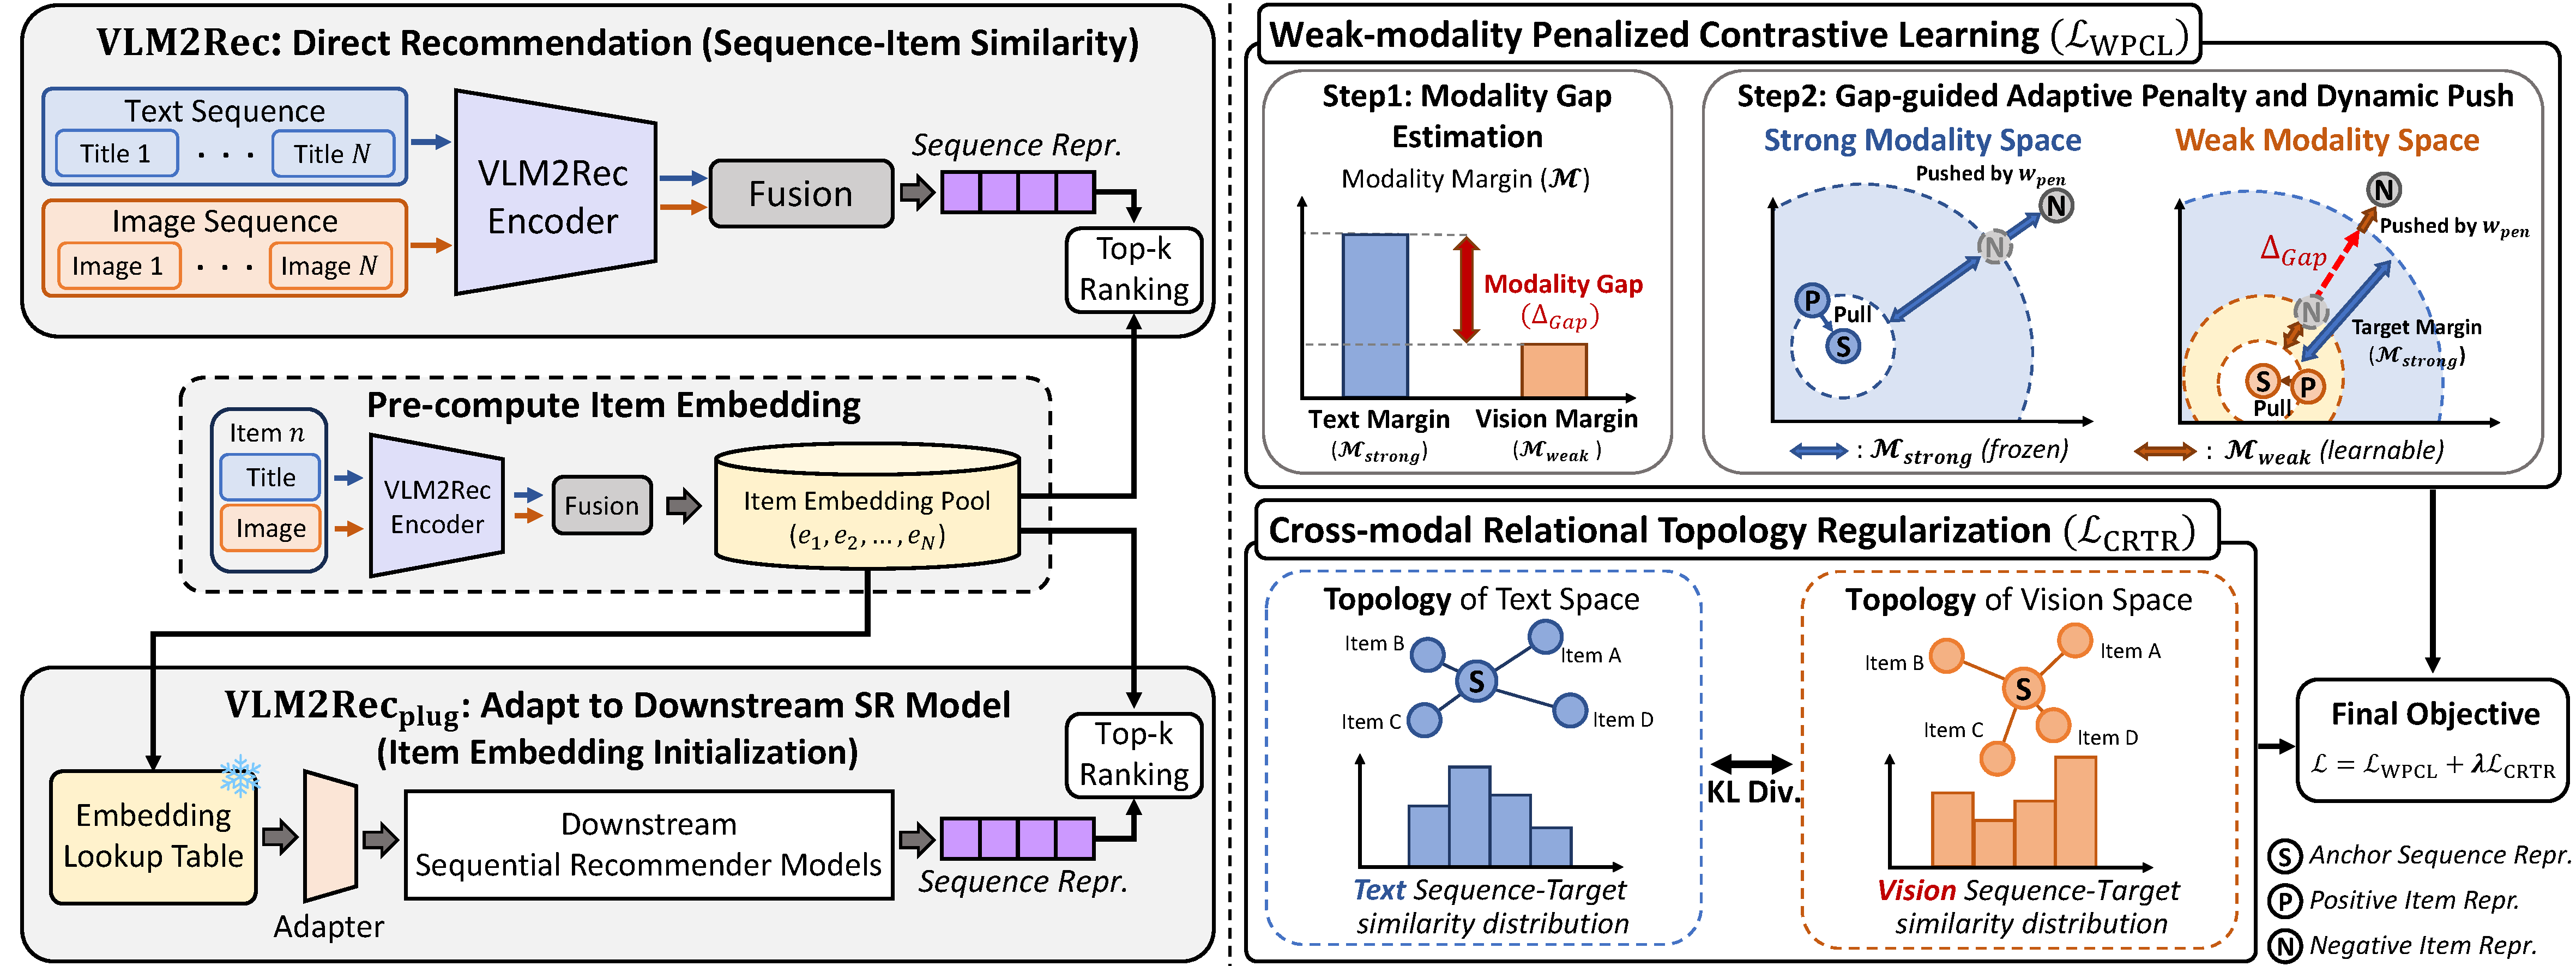
\includegraphics[width=\textwidth]{figures/method_www.pdf}
    \caption{Overview of our framework. Left: VLM2Rec directly ranks items by sequence--item similarity, while $\text{VLM2Rec}_{\text{plug}}$ replaces the item embedding table of a downstream SR backbone with precomputed item embeddings and serves without VLM calls. Right: the shared encoder is trained with $\mathcal{L}_{\text{WPCL}}$ to improve weak-modality discrimination and $\mathcal{L}_{\text{CRTR}}$ to align each user's relational structure across the two modalities.}
    \Description{A unified framework diagram shows direct recommendation with VLM2Rec, downstream SR inference with VLM2Rec plug using precomputed item embeddings, and the shared WPCL and CRTR training objectives.}
    \label{fig:method}
\end{figure*}
% Table: uniformity and separability comparison

\vspace{+0.1cm}
\noindent\textbf{A1: Adding Vision Can Hurt.}
We first examine how standard SFT (Eq.~\ref{eq:sft_loss}) affects modality-specific recommendation performance.
In Fig.~\ref{fig:drop_grad} left, \TEXTset{}, \VISIONset{}, and \FUSIONset{} rank items by the similarity of the text-only ($\mathbf{e}_u^T$), vision-only ($\mathbf{e}_u^V$), and fused ($\mathbf{e}_u$) sequence embeddings to the fused item embeddings $\mathbf{e}_i$.
The Vanilla model ($\text{VLM}_\text{Vanilla}$) already shows a large gap of \TEXTset{} over \VISIONset{} (6.9\% and 7.2\%), reflecting the inherent text-dominant prior of VLMs; yet visual signals can still add complementary preference evidence on some domains (\FUSIONset{}<\TEXTset{} on Beauty but \FUSIONset{}>\TEXTset{} on MovieLens).
However, $\text{VLM}_\text{SFT}$, though necessary to adapt VLMs to SR, worsens this collapse: the \TEXTset{}--\VISIONset{} gap widens to 12.1\% and 14.6\%, and \FUSIONset{} ends up below \TEXTset{} on both datasets. 
Adding visual embeddings now causes negative transfer, lowering next-item accuracy rather than improving it.
To rule out LoRA updates as the cause, we freeze the VLM and train only a linear head with the same loss, and the gap still widens (App.~\ref{app:head_sft_control}).

\vspace{+0.1cm}
\noindent\textbf{A2: SFT Widens the Text--Vision Gradient Gap.}
To examine this degradation, we feed the fused, text-only, and vision-only sequence embeddings into the SFT loss (Eq.~\ref{eq:sft_loss}) and take the gradient with respect to each, denoted by $\mathbf{g}_{\text{fusion}}$, $\mathbf{g}_T$, and $\mathbf{g}_V$. We then measure their alignment $\cos(\mathbf{g}_{\text{fusion}},\mathbf{g}_m)$ for $m\in\{T,V\}$ (Fig.~\ref{fig:drop_grad} right).
This alignment shows how closely the fused gradient follows each modality's own gradient in direction, and we call the difference between the two the \textit{gradient gap} (shaded in Fig.~\ref{fig:drop_grad} right).
From the start, $\mathbf{g}_{\text{fusion}}$ is strongly aligned with the text gradient $\mathbf{g}_T$, while alignment with the vision gradient $\mathbf{g}_V$ drops rapidly.
As SFT pulls each user's sequence embedding toward the next item, $\cos(\mathbf{g}_{\text{fusion}},\mathbf{g}_T)$ rises, whereas $\cos(\mathbf{g}_{\text{fusion}},\mathbf{g}_V)$ only partly recovers and then declines as the imbalance accumulates.
Under SFT, the gradient gap stays large, averaging 0.74 on Beauty and 0.87 on MovieLens over the last 20\% of training (smoothed curves), whereas VLM2Rec closes it ($-0.27$ and $-0.08$).
The large gap under SFT is consistent with the model learning sequence-level CF mainly through the easier text modality as a \textit{shortcut}~\cite{shortcut2}, although these embedding-level gradients do not directly measure each modality's parameter update.




\vspace{+0.1cm}
\noindent\textbf{A3: SFT Sharpens the Text Space, Not the Visual Space.}
To see how this bias shapes the sequence--item representation space used to rank next items, we measure uniformity $U^m$ and alignment $A^m$~\cite{align} between sequence and item embeddings (Tab.~\ref{tab:ali_uni_clo}).
$U^m$ measures how evenly the embeddings spread over the unit hypersphere and approaches 0 as the space collapses, while $A^m_{\text{pos}}$ and $A^m_{\text{neg}}$ measure the squared distance from a user's sequence embedding to the next item and to negatives, respectively:
\begin{equation}
\begin{gathered}
U^{m}
\triangleq
\log
\mathbb{E}_{(u,i)\sim \mathcal{P}_{\text{uniform}}}
\Big[e^{-2\|\mathbf{e}_u^m-\mathbf{e}_i^m\|_2^2}\Big],\\
A_{\text{pos}}^{m} \triangleq
\mathbb{E}_{(u,i^+)\sim \mathcal{D}}
\Big[\|\mathbf{e}_u^m-\mathbf{e}_{i^+}^m\|_2^2\Big],\\
A_{\text{neg}}^{m}
\triangleq
\mathbb{E}_{(u,i^+)\sim \mathcal{D}}
\mathbb{E}_{i^- \sim \mathcal{P}_n(\cdot \mid u)}
\Big[\|\mathbf{e}_u^m-\mathbf{e}_{i^-}^m\|_2^2\Big],
\end{gathered}
\end{equation}
where $\mathcal{D}$ holds evaluation user--next-item pairs, $\mathcal{P}_n(\cdot\mid u)$ samples $u$'s negatives, and $\mathcal{P}_{\text{uniform}}$ samples random sequence--item pairs.
% Since next-item ranking depends on whether the next item lies closer to the user's sequence than negatives do, rather than on absolute alignment, we derive separability $S^m$ from the alignment terms:
Since ranking depends on whether the next item lies closer to the user's sequence than negatives do, not on absolute alignment, we derive separability $S^m$ from the alignment terms:
\begin{equation}
S^m \triangleq A^m_{\text{neg}} / (A^m_{\text{pos}} + \epsilon),
\end{equation}
where $\epsilon$ is a small constant; $S^m>1$ means that, on average, the modality places users' next items closer than negatives, and $S^m$ near 1 means that it barely does so.
As shown in Tab.~\ref{tab:ali_uni_clo}, under SFT the fused space is closer to the text space than to the vision space in both $U^m$ and $S^m$, indicating that text dominates the fused embeddings.
This is consistent with A2: SFT injects sequence-level CF mainly through text, improving the text space and, in turn, the fused space.
However, the visual modality receives little of this CF signal: its separability stays near 1, far below that of text, and its uniformity lags behind text, indicating collapse in the visual sequence--item space.

\vspace{+0.1cm}
\noindent\textbf{Summary.}
Overall, SFT amplifies the modality collapse that is already present in VLMs.
Its fused gradient mostly follows the text gradient, and the weak visual modality's representation space collapses further, which widens the text--vision accuracy gap and causes negative transfer when fused.
The same pattern appears on Toys and the visually informative Clothing domain (App.~\ref{app:additional_analysis}), and SFT leaves a sizable \TEXTset{}--\VISIONset{} gap across VLM families and scales (Tab.~\ref{tab:modality_collapse_backbones}).